\documentclass[11pt,a4paper]{article}
\usepackage[utf8]{inputenc}
\usepackage[spanish]{babel}
\usepackage{amsmath}
\usepackage{amsfonts}
\usepackage{amssymb}
\usepackage{graphicx}
\usepackage{url}
\author{Ignacio Ram\'{\i}rez}
\title{Clasificación de tipos de documento}

\begin{document}

\maketitle

\section{Descripción del problema}

Se trata de clasificar (agrupar) los documentos según diferentes \emph{tipos}, pero sin tener esos tipos identificados de antemano, es decir, es un problema de agrupación no supervisada (o clustering). 

El lograr una buena agrupación facilitaría muchísimo otros aspectos del procesamiento previo a LUISA así como del posterior de los resultados.

La figura~\ref{fig:docs} muestra algunos ejemplos de distintos posibles tipos de documentos. Algunos son cartas, otros son formularios, otros son recortes de diario, etc.

\begin{figure}
\centering%
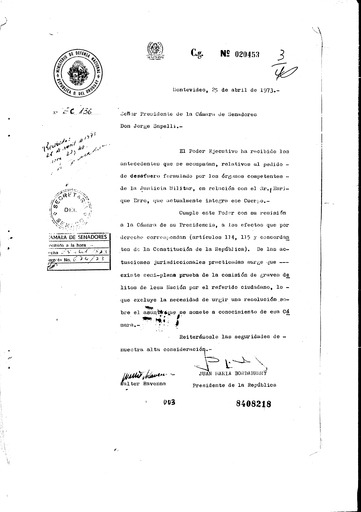
\includegraphics[width=0.49\textwidth]{r0566_0011.jpg}%
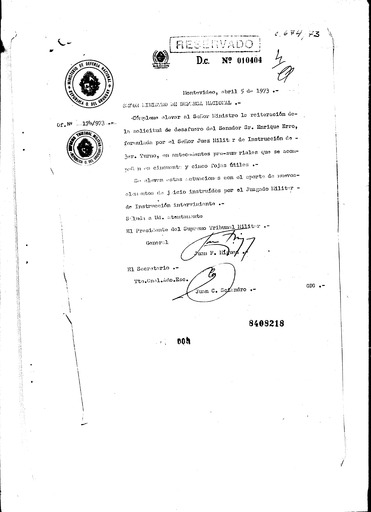
\includegraphics[width=0.49\textwidth]{r0566_0012.jpg}\\
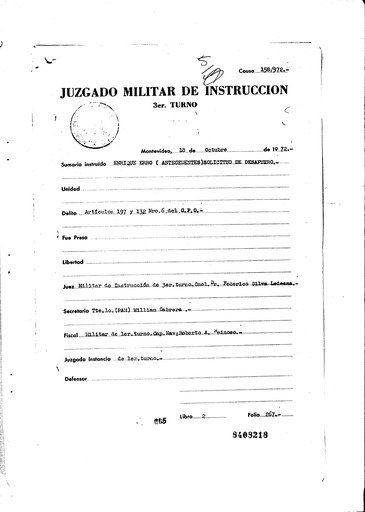
\includegraphics[width=0.49\textwidth]{r0566_0013.jpg}%
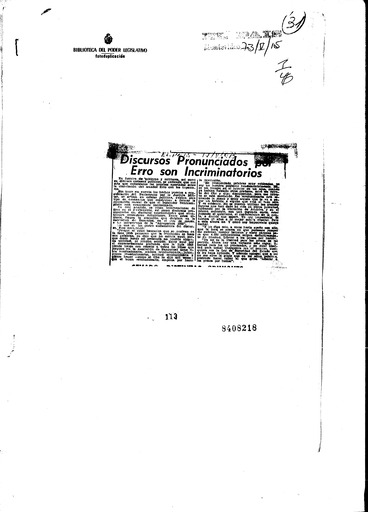
\includegraphics[width=0.49\textwidth]{r0566_0121.jpg}\\
\caption{\label{fig:docs}Ejemplos de distintos tipos de documento (hay muchísimos más!). La idea es identificar el tipo de acuerdo a su \emph{aspecto general} más que a su contenido textual, que no está disponible.}
\end{figure}

\section{Consideraciones técnicas}

Este es un problema abierto y como tal tiene mucho trabajo de investigación, ensayo y error.

La idea es que el método sea razonablemente rápido. Las formas en que hemos atacado este problema hasta el momento (sin una solución elegida en particular) es identificar rasgos generales de los documentos a nivel visual, como ser \emph{textura} o variaciones globales de la intensidad a lo largo del documento. Ideas como la de los perfiles de intensidad de las filas que se aplican para alinear pueden servir aquí. Hay que ser creativos.

\end{document}